% Chapter Template

\chapter{Introduction} % Main chapter title

\label{Chapter1} % Change X to a consecutive number; for referencing this chapter elsewhere, use \ref{ChapterX}

\lhead{Chapter 1. \emph{Introduction}} % Change X to a consecutive number; this is for the header on each page - perhaps a shortened title

%----------------------------------------------------------------------------------------
%	SECTION 1
%----------------------------------------------------------------------------------------

%############################# Introduction #################################
\section{Background}
  Concrete is the synthetic material currently produced in volumes larger than any other material on Earth. With an annual consumption of approximately 35 billion tonnes, it is only second to water in terms of global usage\supercite{Monteiro2017, VanDamme2018}. As the backbone of modern infrastructure, it provides the foundations for buildings, bridges, roads, dams, and other structures essential for societal development. Its widespread adoption arises from a unique combination of strength, versatility, and cost-effectiveness\supercite{Mehta2014}, rendering it indispensable to the construction industry.


  Nevertheless, despite the ubiquity of concrete, the properties of its key constituent, cement, remain incompletely understood. Cement is a chemically complex material, composed of a heterogeneous mixture of minerals that undergo a series of hydration reactions upon contact with water. The principal product of cement hydration---and the primary binding phase of concrete--- calcium silicate hydrate (C-S-H)\footnote{Cement chemistry nomenclature} is the responsible for the mechanical strength, chemical and transport properties and durability of hardened cement paste and, consequently, of concrete itself\supercite{Papatzani2015, Ioannidou2016, Qomi2020, Bahraq2022}. Therefore, understanding the atomic and mechanical properties of C-S-H is of the uttermost importance to better formulate cementitious materials with enhanced performance and durability.\supercite{Foley2012}

  In the last two decades, significant efforts have been made to 


\begin{figure}[H]
    \centering
    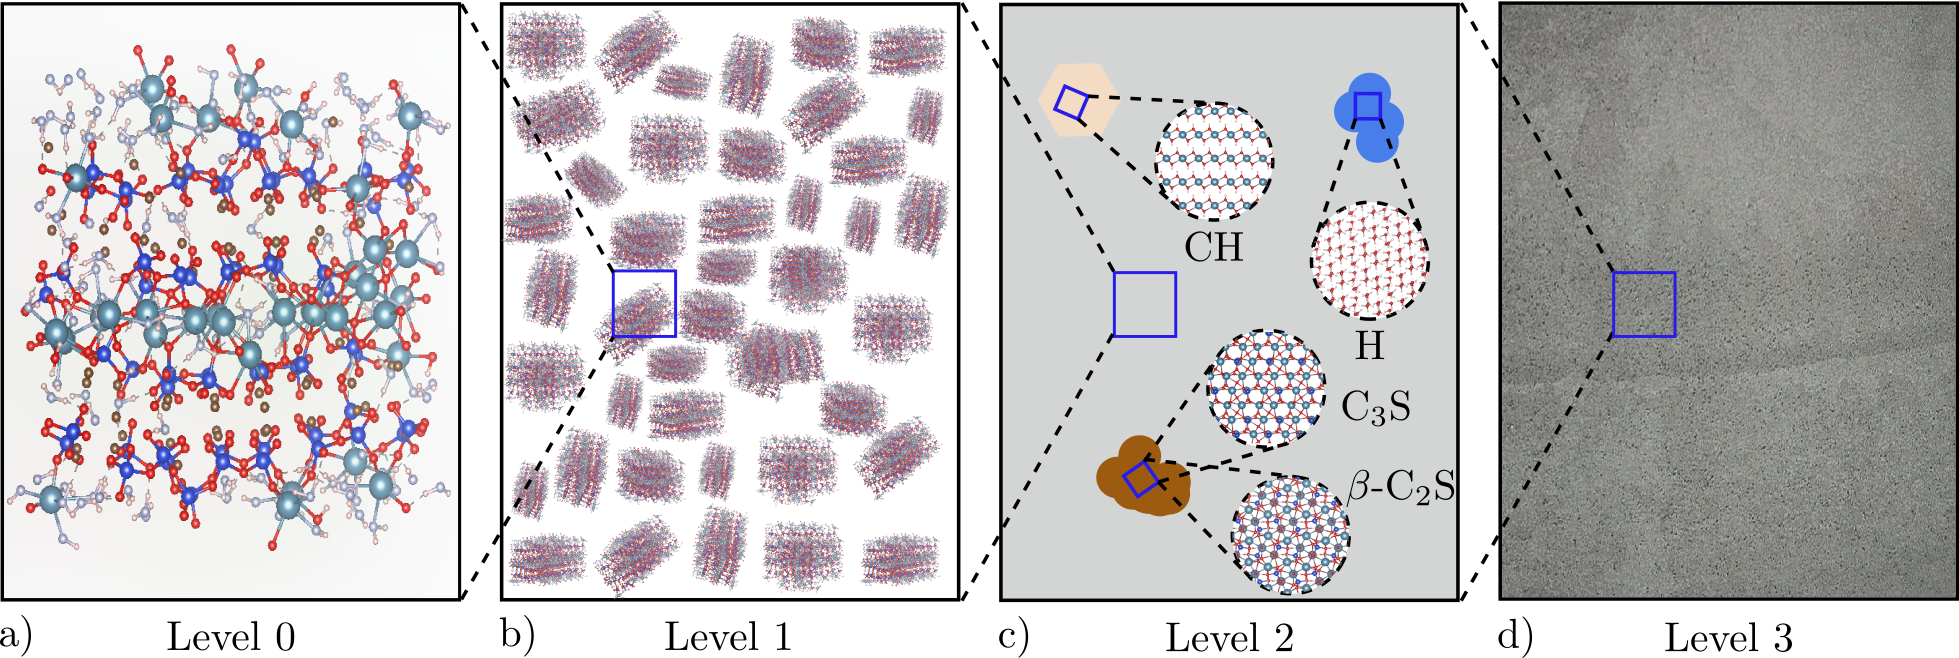
\includegraphics[width=0.9\textwidth]{levels.png}
    \caption{A four-level model representing the upscaling of C-S-H properties from the nanoscale to the engineering scale. (a) snapshot of C-S-H's nanostructure. (b) microstructure of C-S-H created by agglomeration of randomly oriented C-S-H nanoparticles. (c) microtexture of hardened paste composed by hydration products. (d) macrotexture of cement paste at the engineering scale. Adapted from \supercite{AbdolhosseiniQomi2015}.}
    \label{fig:figure1}
\end{figure}
%-----------------------------------
%	SUBSECTION 1
%-----------------------------------
\section{Problem Statement}


%-----------------------------------
%	SUBSECTION 2
%-----------------------------------

\section{General and Specific Objectives}

%----------------------------------------------------------------------------------------
%	SECTION 2
%----------------------------------------------------------------------------------------

\section{Overview}




